%!TEX root = ../index.tex

% 
% Architecture
% 

\section{Architecture}

In this section we describe our proposed architecture for the remaining implementation work. The software stack is composed by several subsystems that have one specific goal, exposing a well known API, this way the subsystems become interchangeable. These subsystems include:

\begin{itemize}
  \item \textbf{Communication service} - Responsible for routing messages between nodes in the DHT.
  \item \textbf{Service router} - Processes the messages that have as destiny the its node, the goal is to call the right service (storage, reputation mechanism, job execution, etc) accordingly. One other key aspect is the ability to attach new services during the runtime.
  \item \textbf{Storage service} - Stores any data that requires persistence in the network, such as job logs, reputation logs and file meta data and chunks.
  \item \textbf{Job coordination} - A subsystem responsible for coordinating jobs requested by the client, keeping state and assuring its completion/
  \item \textbf{Job execution} - Execution of jobs, gathering all the necessary assets (image processors, sound wave manipulators, etc) to complete the job/
  \item \textbf{Reputation Mechanism} - Validate user behavior and right to take different responsibilities in the network.
  \item \textbf{Client API and CLI} - In order to interact with the network, we offer an API and a CLI with Unix type instructions and familiar web cloud instructions that developers are familiar.
  \item \textbf{Rendezvous points} - The only centralized component in this architecture, its purpose is for the clients to have a way to connect to the overlay network. 
\end{itemize}


In the following section we present the proposed components of the architecture using a `bottom up' approach, starting with the software architecture of each node in section 4.1, moving into how the network is structured and how the nodes can join the network, described in section 4.2, ending with an specification of how to intersect with browserCloud.js, thorough an RESTful API endpoint or using a Command Line Interface (CLI). We present how this components are connect with each other in Figure~\ref{fig:softwarestack}.

\begin{figure}[h!]
  \centering
  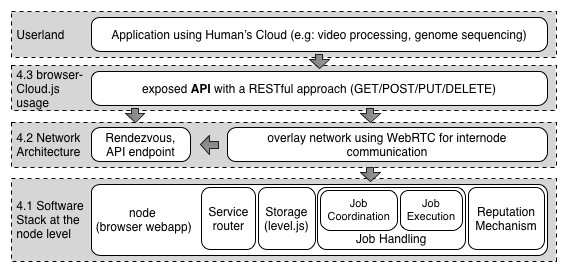
\includegraphics[width=\textwidth]{img/softwarestack.jpg}
  \caption{browserCloud.js overall architecture}
  \label{fig:softwarestack}
\end{figure}


\subsection{Software Architecture at the node level}

At the node level, we divide the application into two fundamental services and three pluggable components, with the possibility for expansion, thanks to Javascript dynamic runtime, we can find this structure in Figure~\ref{fig:hcnode}.

In the communication layer, we find the DHT logic implemented to effectively propagate messages. One of the main goals with component is to be modular, so we can switch between different DHT algorithm if necessary, without affecting the rest of the application functionality.

Next, we have the Service Routing layer, this service is responsible to guide the message to the right component, enabling the architecture to be more modular, plugging in more components as it is needed. For example, when a node ascends and needs the storage component to fulfill his responsibility.

Last, we have the components, individual modules that do one thing and one thing well. Currently, we present the Storage module, responsible for holding the data; the Job Scheduler, responsible to orchestrate jobs issued by the users; the assets needed to execute the jobs and finally; the job executor, the module that will execute the jobs in a separate process using webworkers.



\begin{figure}[h!]
  \centering
  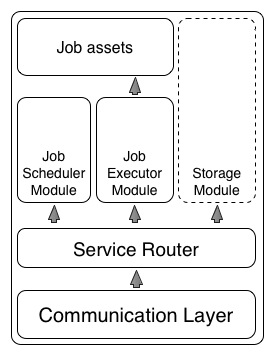
\includegraphics[width=0.35\textwidth]{img/node.jpg}
  \caption{browserCloud.js Node}
  \label{fig:hcnode}
\end{figure}

\subsubsection{4.1.1 Storage -}

browserCloud.js storage happens in what it is named, the ``Ascended node ring'', these nodes have an higher reliability, making the storage system more stable, without the need of constantly burning computer cycles to maintain the files replica level.

Data stored in nodes can be:
\begin{itemize}
  \item File metadata (name of the file, size, location of the chunks, chunks hash);
  \item File chunks;
  \item Directories metadata - This way, bcls can be more efficient ;
  \item Job information (state, issuer, workflow);
  \item Reputation log;
\end{itemize}

We classify storage nodes into two types: 1) the `sKeeper', responsible for holding the metadata of the file and hashing each chunk to identify the `sHolder'; 2) `sHolder' nodes responsible to store the chunk into their system. This approach mitigates the possibility of having an highly unbalanced storage distribution, dividing each file in equal chunks across several nodes. As we can see in Figure~\ref{fig:chunking}, each chunk gets hashed more than one time with a different hash function, its purpose being to identify several Nodes that will be responsible to store a replica of the chunk. Also, in order to increase the fault tolerance of the system, we replicate the `sKeeper' responsibility in the two following nodes in the hashring, so if one of these fails, another is assigned.

\begin{figure}[h!]
  \centering
  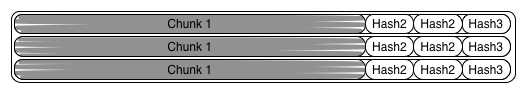
\includegraphics[width=0.7\textwidth]{img/chunking.jpg}
  \caption{A file partitioned in several chunks, each with its corresponding hashes that correspond to nodeIds}
  \label{fig:chunking}
\end{figure}

In Figure~\ref{fig:skeepersholder}, we can find the `sKeeper' and `sHolder' relationship. Only the sKeeper performs the chunk hashing and stores the information in the file lookup table. This happens one single time for each chunk, reducing several network hops per message on the consequent searches.

\begin{figure}[h!]
  \centering
  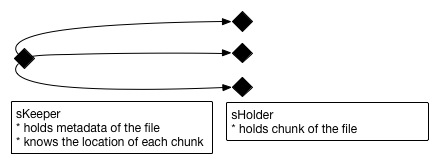
\includegraphics[width=0.7\textwidth]{img/skeepersholder.jpg}
  \caption{Representation of the Node responsible for the file(sKeeper) and it's individual chunk holders(sHolders)}
  \label{fig:skeepersholder}
\end{figure}

Each store file is chunked as soon as it enters the network, thus mitigating the risk that would be present if we were transferring files with considerable sizes all at once, starving the network and the node's heap. The only point where the file gets assembled together again is when it leaves the network and sent to the user, and even this could be made to perform chunk transfer in parallel to the client directly.

browserCloud.js adapts the Load Balancing virtual server's method, by using the same strategy of global load, but by transferring files between sHolders and not an entire virtual server, updating the respective sKeeper accordingly. Files are storage as objects in a indexedDB type storage, provided by the leveljs module.

\subsubsection{4.1.2 Distributed Job Scheduling -}

Job coordination is one of the main challenges in a completely distributed environment, in a sustainable and scalable way. Traditionally in the client-server model, we have the possibility to select one of the nodes to be the job coordinator. To implement this in a P2P network, we take advantage of the DHT, to select randomly one of the ascended nodes to be the `jKeeper', the node responsible for coordinating the job in an environment a P2P network.

The `jKeeper' is responsible for contacting the `sKeepers' of each individual file, and coordinate them to command each of `sHolder' to perform the desired computation on the file. All the steps during the computation are journaled in the Job log, stored with the coordinator, and replicated in the two following nodes for Fault Tolerance measure.

All the coordination takes place in the ascended Node ring, however, in order to take advantage of the normal node ring resources. `sHolders' are allowed to offload the computation to process this job in the `normal hash ring'. This is done by sending a probe, asking for `volunteers' for a job, when the threshold required is met, the orchestration starts, where the `sHolder' transfers the data and the assets necessary for processing it.

An example in pseudo-code can be analyzed below: \\

\textit{Client pseudo-code}
\begingroup
\scriptsize
\begin{verbatim}
var jobId = randomUniqueIdGenerator();
sendJob(jobId, job); // job object includes the files names being manipulated+assets
\end{verbatim}  
\endgroup



\textit{jKeeper pseudo-code}
\begingroup
\scriptsize
\begin{verbatim}
var jobLog = createNewJobLog();
replicateJob(jobLog); // each job replica holder will ping the jKeeper to make sure progress 
// is made, if the node fails, other will assume its role
job.sKeepersList.forEach(function (sKeeper){
  commandJobExecution(job, sKeeper, statusReport);
  function statusReport(status){
    jobLog.log(status);
  }  
}); //Job is complete
\end{verbatim}
\endgroup

\textit{sKeeper pseudo-code}
\begingroup
\scriptsize
\begin{verbatim}
var sHolders = this.getsHolders(job.filename);
sHolders.forEach(function(sHolder){
  commandTaskExecution(sHolder, taskReport);
  function taskReport(status){
    reportBack(status); // report to jKeeper
  }
});
\end{verbatim}
\endgroup

\textit{sHolder pseudo-code}
\begingroup
\scriptsize
\begin{verbatim}
if(smallTask && available) {
  doIt(task, taskReport);
} else {
  requestNormalNodesToExecute(task, taskReport)
}
function taskReport(status){
  reportBack(status); // report to sKeeper
}
\end{verbatim}
\endgroup

\subsubsection{4.1.3 Reputation Mechanism -}


The reputation mechanism present will enable the network to identify the nodes that show more availability and have the necessary means to ascend and take a more important role. In order to evaluate each node, we define several metrics, these are: uptime, number of job completions, network throughput and computational resources (CPU) available, being the uptime, the most important, to assure stability. The reputation metric is calculated as follows: \\

$ \textbf{reputation} = \alpha * log(uptime) + \beta * log(job completions) + $ \\
$          \gamma * log(network throughput) + \delta * log (CPU)$
\\
where: \\
\\
  $\alpha+ \beta+ \gamma+ \delta = 1$; \\
  $\alpha > \beta + \gamma + \delta$;  \\

We chose to normalize the metrics and give more importance to the uptime of the system, because this is the one metric allowing a more stable network for storage.

The reputation of each node is stored with its node identifier on the `ascended hash ring'. Each time a job is completely successfully, this score gets updated and in case it reaches the required level to ascend, the jKeeper that was updating thus score will enable and deploy the remaining features (storage and job schedule module) it needed to join the ascended group. 

\subsection{Network Architecture}

We designed browserCLoud.js network architecture as shown in Figure~\ref{fig:overallarchitecture}, being composed by 4 different elements, being:

\begin{itemize}
  \item Normal Nodes - We refer to normal node as the node responsible for only computation task in our network.
  \item Ascended Nodes - These nodes are responsible for both computation, storage and job coordination.
  \item API endpoints - The rendezvous points for the browsers to download the necessary code to enter in the browserCloud.js network. These API endpoints are also responsible for establishing the connection from a client to a browser.
  \item Clients that use browserCloud.js - Applications using the RESTful API to interact with browserCloud.js
\end{itemize}

\begin{figure}[h!]
  \centering
  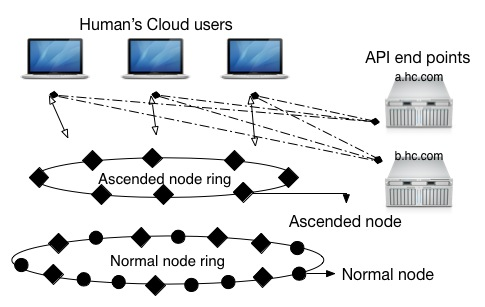
\includegraphics[width=0.8\textwidth]{img/overall.jpg}
  \caption{browserCloud.js network architecture}
  \label{fig:overallarchitecture}
\end{figure}


\subsubsection{4.2.1 Structured Overlay Network -}

Nodes are divided into two Chord DHTs with the purpose of separating the nodes with storage and job coordination responsibility responsibility from the ones with only computing responsibility. The reason behind this decision is due to the high churn rate in a P2P network. Keeping the files in nodes that have proven to be more trustworthy for staying longer in the network makes the system more robust, keeping the file replica level stable. This also reduces the message overhead that would require to keep the replica level in a more inconsistent environment. Nevertheless, the more volatile nodes are perfect for short computing operations, till they proven to be trustworthy to `ascend' in the network.


\subsubsection{4.2.1 Rendezvous points -}

Since browsers cannot effectively have a static IP nor have a DNS record updated on demand pointing to themselves, we designed the API endpoints as the rendezvous between browsers and clients, so the connection can be established.

\subsection{browserCloud.js usage}

The client API goal is to be familiar to experienced developers using cloud providers today and at the same time, respect the Unix philosophy, where the job work flows are composed by a stream of assets, that do one thing and one thing well. It will support CRUD operations through a REST with JSON API, a filesystem-like interface (directories and objects), where user is identified by a username and it maps to the paths shown in Table~\ref{tbl:dirrepnet}: 

\begin{table}
  \centering
  \begin{tabular}{ p{3cm} | p{12cm} }
  % \hline 
  Path & Description \\
  \hline 
  /:username/jobs/ & where new jobs can be inserted by the user \\
  \hline
  /:username/jobs-reports/ & Job status. The user is only able to read and delete the records, they are created by the system. \\
  \hline 
  /:username/home/ &  Private user store, only place where the user has write access \\
  \hline   
  /:username/reports/ & Usage and Access log reports. \\ 
  \hline   
  /nodes/ & Registry of all the nodes in the network with their metadata, the user can only read this folder. \\
  % \hline   
  \end{tabular}
  \caption{Directories representation inside the network}
  \label{tbl:dirrepnet}
\end{table}

\subsubsection{4.3.1 Application Programming Interface (API) -}

We provide a REST API for the developer to use. The reason behind this design decision is to create a familiar interface to the majority of web developers. The server replying to these requests defined in Table~\ref{tbl:restapi}, can be a public or a private proxy, in the user machine, behind a company firewall or as a public service available to the community. Thus, it remains portable and does not lock in the user to a provider.

\begin{table}[h!]
  \centering
  \begin{tabular}{ l | c | p{12cm} }
    \multicolumn{3}{ l }{\textbf{Directories}} \\
    Action: PutDirectory & \multicolumn{2}{l}{PUT /:username/home/[:directory]/:directory} \\
    Action: ListDirectory & \multicolumn{2}{l}{GET /:username/home/[:directory]/:directory} \\
    Action: DeleteDirectory & \multicolumn{2}{l}{DELETE /:username/home/[:directory]/:directory} \\
    \hline 
    \multicolumn{3}{ l }{\textbf{Files}} \\
    Action: PutFile & \multicolumn{2}{l}{PUT /:username/home/[:directory]/:filename} \\
    Action: GetFile & \multicolumn{2}{l}{GET /:username/home/[:directory]/:filename} \\
    Action: DeleteFile & \multicolumn{2}{l}{DELETE /:username/home/[:directory]/:filename} \\
    \multicolumn{3}{p{15cm}}{\textbf{Note:} PutFile and GetFile, the body of the request and response  respectively is the file} \\
    \hline 
    \multicolumn{3}{ l }{\textbf{Jobs}} \\
    Action: CreateJob & \multicolumn{2}{l}{PUT /:username/jobs} \\
    Action: CancelJob & \multicolumn{2}{l}{DELETE /:username/jobs/:jobId} \\
    Action: ListJobs & \multicolumn{2}{l}{GET /:username/jobs} \\
    Action: GetJob & \multicolumn{2}{l}{GET /:username/home/jobs/:jobId} \\
    Action: GetJobOutput & \multicolumn{2}{l}{GET /:username/jobs-reports/:jobId} \\
    \hline \\
    \multicolumn{3}{p{15cm}}{\textbf{Note:} Create Job, several arguments are passed, most importantly, an array named ``phases'' that includes the orders with assets necessary in order to execute the job(e.g. `grep -ci' or if its a new asset, it should be a JS object with a closure.)} \\
    \hline 
  \end{tabular}
  \caption{browserCloud.js REST API Draft}
  \label{tbl:restapi}
\end{table}

\subsubsection{4.3.1 Command Line Interface (CLI) -}

We are also including a CLI\footnote{CLI - Command Line Interface} tool to enable quickly bash scripts for computation jobs and file storage, this CLI uses in the background the API defined in Table~\ref{tbl:restapi}. For example, if we are looking for video transcoding: ``hcjob create /path/to/file | ffmpeg | /path/to/out.webm''. The rest of the commands are:
  
\begin{itemize}
  \item \textbf{\$ bcls}  - List files in a directory
  \item \textbf{\$ bcget} - Get an object stored
  \item \textbf{\$ bcput} - Store an object
  \item \textbf{\$ bcjob} - Initialize a job   
\end{itemize} 

% 
% \subsection{Class Diagram}
% 